\chapter{METODOLOGIA}
\label{metodologia}

Será mostrado neste capitulo os materiais, ferramentas e métodos utilizados na realização deste trabalho. Em detalhes, são explicados a constituição e captação dos bancos de sinais neurais, métodos de processamento por injeção de banco de dados no algoritmo, o jogo utilizado como exemplo e as métricas utilizadas para avaliar o trabalho. \todo{listar todo o conteúdo deste capitulo quando o trabalho for finalizado}

\section{Materiais}

\subsection{Banco de Sinais Neurais e Fisiológicos}
Para esse trabalho utilizamos dados que contemplem, de alguma forma, o estado emocional de pessoas dentro de um contexto. Esses dados podem ser encontrados, nas metodologias investigadas na forma de sinais eletromagnéticos "crus" vindo de regiões conhecidas e pré estabelecidas do cérebro.

Uma das formas menos invasivas e melhor desenvolvidas para captação desses sinais é o Eletroencefalograma (EEG). Esse método consiste na utilização de eletrodos para captação de pulsos eletro-magnéticos do cérebro em determinadas regiões que, a depender do tipo de estimulo e feedback verbal do estado emocional reportado por um participante no momento da coleta, serão classificados como positivos ou negativos.

No caso deste trabalho, foram utilizados os bancos \cite{linkbase1} e \cite{linkbase2} que contem dados captados das formas mencionadas para treinar um algoritmo de reconhecimento de padrões. \todo{detalhar melhor os pormenores dos bancos}

\section{Métodos}

% Foram pensadas em duas metodologias levemente distintas em relação a captação dos dados e em como serão utilizados.

% \subsection{Detecção e Feedback Simultâneos}
% A primeira, chamado "Método com detecção e feedback simultâneos" parte do principio que a detecção dos dados, ou seja, a captação dos sinais neurais, ocorrerá ao mesmo tempo que a interpretação e utilização desses dados dentro do jogo. Este é um cenário ideal onde o loop de feedback é fluidamente realizado: o jogador, ao jogar o jogo, gera sinais que, ao serem interpretados pelo algoritmo fazem com que o jogo se adapte passivamente a esses sinais. Com isso, o jogador reage a essa adaptação, gerando um novo fluxo de sinais, e assim sucessivamente. Essa metodologia, além de depender de todos os equipamentos e programas para captação e interpretação correta de sinais, é também um grande desafio de performance e paralelismo.

% \begin{figure}[h]
%     \centering
%     \caption{Diagrama de Metodologia Paralela}
%     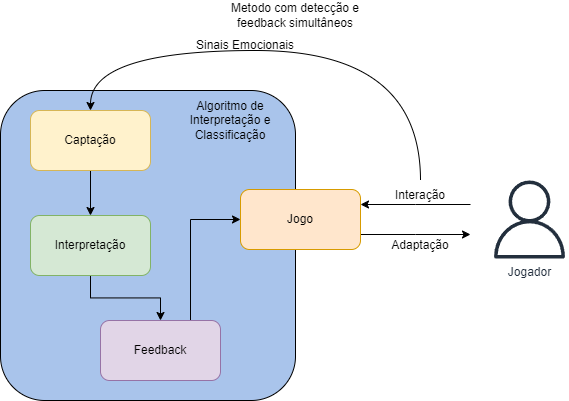
\includegraphics[width=10cm]{Figuras/diagrama-metodologia-um.drawio.png}
%     \caption*{Fonte: Autores}
%     \label{fig:diagrama_metodologia}
% \end{figure}

\subsection{Injeção de Banco de Dados}
Este método é levemente simplificado no setor de pré-interpretação com relação a uma leitura ao-vivo utilizando equipamentos de sensores EEG. Ao invés de ser utilizada a captação ao mesmo tempo que a interpretação dos dados, foi utilizado um banco de dados já classificado e conhecido. Esses dados foram injetados em um algoritmo treinado para sua interpretação e imediata utilização pelo jogo. Dessa forma, ao invés de estarmos testando a verdadeira saída emocional do jogador, focamos na capacidade do algoritmo de interpretação e do jogo de agirem ao mesmo tempo através da injeção dos dados de uma base conhecida no algoritmo. \todo{detalhar melhor o que tem na base de dados}

\begin{figure}[h]
    \centering
    \caption{Diagrama de Metodologia Classificada}
    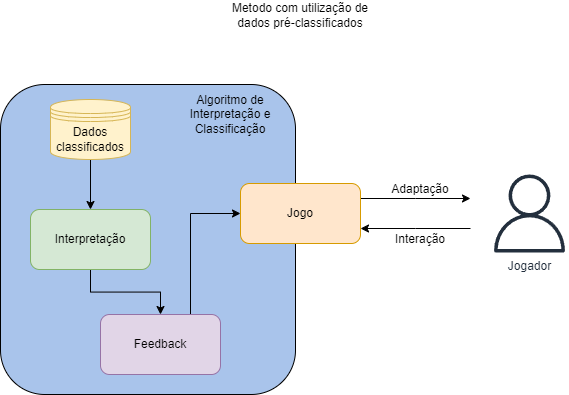
\includegraphics[width=10cm]{Figuras/diagrama-metodologia-dois.drawio.png}
    \caption*{Fonte: Autores}
    \label{fig:diagrama_metodologia}
\end{figure}

Foi optado por essa metodologia por conta da necessidade de permissões para utilizar um método que realizasse a leitura através de equipamentos de EEG durante a execução do jogo em voluntários, mas também para que o foco do trabalho seja a adaptabilidade de um sistema - nesse caso, o jogo - quando utilizada essa entrada de dados. \todo{rever a parte sobre o foco deste trabalho, a depender do desenrolar do projeto}

\subsection{Jogo}
O jogo que utilizamos como base é uma versão modificada dos projetos realizados durante as aulas de Desenvolvimento de Jogos Digitais no sétimo ciclo do curso. Se trata de um jogo de plataforma no estilo de clássicos como \textit{Castlevania} \cite{castlevania} e \textit{Super Metroid} \cite{supermetroid}, melhor detalhado a frente.

\todo{descrição do jogo do projeto. não é versão final.}
No jogo deste projeto, o jogador controla um personagem capaz de se transformar a depender da emoção do jogador. Ao se transformar, as mecânicas do jogo se alteram, mudando como o jogador deve jogar o jogo e as reações do mundo do jogo ao personagem.

O jogo passou por adaptações de compatibilidade com o algoritmo de classificação em tempo real que será desenvolvido, tanto para receber os dados como para implementar as diferentes mecânicas adaptativas.

O jogador pode jogar e testar as novas funcionalidades, por meio de inputs programáveis que serão disponibilizados no jogo. Esses inputs, através de botões, simularão a inserção da emoção do jogador, pois não é permitido captar diretamente as ondas transmitidas pelo usuário.

\section{Métricas}

Como métrica, após o teste das duas diferentes versões do jogo: com sistema de adaptabilidade e sem sistema de adaptabilidade, foi realizado um questionário com perguntas a cerca da satisfação dos jogadores comparando as duas versões. As perguntas giram em torno de três aspectos: 

\begin{itemize}
  \item Satisfação com as Mecânicas: o quanto a mudança de mecânicas agrada com relação as mecânicas padrões não-adaptativas do jogo;
  \item Satisfação com a Imersão: o quanto o jogador se sente mais imerso com relação a imersão sentida na versão não-adaptativa do jogo;
  \item Satisfação Geral: o quanto o jogador gosta mais ou menos do jogo com o sistema adaptativo com relação ao jogo sem o sistema.
\end{itemize}

Essas perguntas foram respondidas em uma escala de -5 a 5, onde -5 é muito menos e +5 é muito mais.

Além disso, foram avaliados o desempenho de algoritmos de leitura de bancos de dados com sinais neurais e fisiológicos, com relação ao tempo de execução, leitura e saída dos dados, para descobrir a viabilidade de sua utilização em simultâneo à execução do jogo. \todo{como será feito?}

